\chapter{Introduction}\label{ch:introduction}

\section{Motivation}\label{sec:motivation}



\subsection{The Importance and Complexity of Systems Engineering}

Many have sought to define what Systems Engineering is:
\begin{enumerate}
    \item \textbf{INCOSE SE Handbook:} ``Systems engineering is a transdisciplinary and integrative approach to enable the successful realization, use, and retirement of engineered systems, using systems principles and concepts, and scientific, technological, and management methods'' \cite{incose_guide_2025}.
    \item \textbf{ISO/IEC/IEEE 15288:} ``An interdisciplinary approach governing the total technical and managerial effort required to transform a set of stakeholder needs, expectations, and constraints into a solution and to support that solution throughout its life'' \cite{standard_ieee_15288_2023}.
    \item \textbf{NASA SE Handbook:} ``A methodical, disciplined approach for the design, realization, technical management, operations, and retirement of a system'' \cite{nasa_nasa_2007}.
\end{enumerate}
While the field has not converged on a single canonical definition, these authoritative sources share common themes: systems engineering is inherently \textit{complex}, \textit{high-impact}, and \textit{resource-intensive}.

It is complex because capturing all of the knowledge, relationships, and inter-dependencies between systems---along with the resulting interactions across the Rumsfeld matrix of known-knowns, known-unknowns, unknown-knowns, and unknown-unknowns---is inherently difficult.

Systems engineering is high-impact because the discipline is responsible for ensuring the integration of systems that are already complex, in addition to mitigating emergent behavior between the systems, they must also try and meet performance, budget, and schedule constraints through a lifecycle. Empirical research show that the "\ac{se} effort has a significant, quantifiable effect on program success with correlation factors as high as 80\%" \cite{walden_systems_engineering_handbook_2015, elm_business_2012, honour_value_systems_engineering_2012}

%% Shows cost accured across the lifecycle 
\begin{figure}[h] 
    \centering
    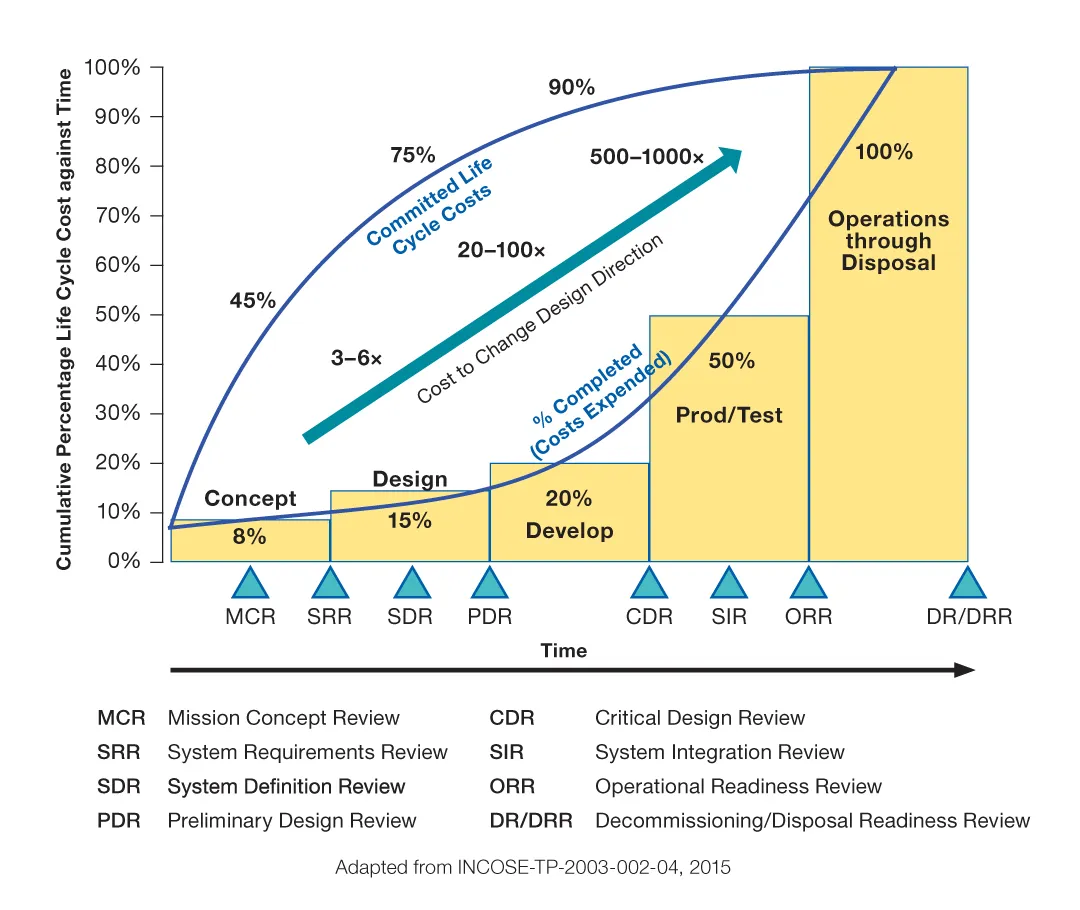
\includegraphics[width=0.8\linewidth]{figs/ch1/lifecycle-cost.png}
    \caption{Life Cycle Cost Impacts \cite{nasa_seh_cost_effectiveness_2025}}
    \label{fig:lifecycle_cost_impacts}
\end{figure}

Poor \ac{se} effort increases lifecycle cost by factors of 10--100$\times$ when defects propagate downstream, while strong \ac{se} effort compresses cost, accelerates timelines, and reduces rework \cite{walden_systems_engineering_handbook_2015, nasa_nasa_2007}.

As programs grow in scope---spanning multi-domain kill chains, autonomous platforms, digital twins, and distributed architectures---the cognitive load on systems engineers increases nonlinearly. Capturing complex system-of-systems interactions, emergent behaviors, and unknown-unknowns becomes increasingly difficult. Tools like \ac{mbse} have emerged to help manage this complexity, but they introduce their own challenges: evolving language standards (SysML v1.x to SysML v2), and the mindset shift from document-centric to model-centric approaches \cite{dau_model-based_2024, delligatti_sysml_2013}. Human bandwidth, coordination overhead, and documentation burdens remain limiting factors, even as \ac{mbse} raises the ceiling for what is possible.

There has to be a better way to help capture and present the complexity in digestible formats to allow systems engineers to continue to make informed architectural decisions. One promising avenue is \ac{ai}. \ac{ai} can help cover more ground, synthesize vast amounts of technical documentation, and augment human reasoning. But how can we ensure that it performs reliably? How can we trust its output? Without such assurance, we might be worse off than we were without it.

\subsection{AI Productivity Potential and Cross-Domain Adoption Benefits}

\subsubsection{Introduction to Large Language Models}




\acp{llm} are advanced artificial intelligence systems trained on massive datasets of text to understand and generate text. These models leverage neural network architectures, particularly transformer-based architectures like \ac{gpt}, to capture syntactic structures, semantic nuances, and pragmatic contexts \cite{vaswani_attention_2017}. When trained on an extensive corpus of text, \acp{llm} have proven themselves capable of approaching average human performance \cite{lab42_about_2024}. When training on more tailored and pruned sources, \acp{slm} have also proven to be quite capable \cite{microsoft_phi_2025, meta_llama3.2_2024, myrzakhan_open_llm_leaderboard_2024}. 

Such capability has effectively unlocked the potential for humans to shift their focus to more abstract, conceptual thought and leave tedious, automatable tasks to machines. The ability to quickly sort through mountains of data proves to be an indispensable tool for domains like systems engineering where legacy, document-centric processes are still heavily represented \cite{estefanSurveyModelBasedSystems2008, harvey_document_model_dont_model_document_2012}. The transformation from document-centric processes to model-centric processes will be heavily enabled through the usage of \ac{ai} tools---leaving only a mindset shift to be required \cite{dod_digital_engineering_strategy_2018, dod_digital_modernization_strategy_2019, simms_adoption_of_de_within_dod_2022, jones_digital_systems_engineering_transformation_strategy_2020}.

Within systems engineering, \acp{llm} augment tasks such as requirement refinement, documentation generation, and systems modeling. For instance, \acp{llm} can analyze initial drafts of requirements or design outlines, clarify ambiguities, improve coherence, and ensure consistent terminology. These capabilities relieve engineers of tedious editing tasks, enabling them to focus on strategic decision-making \cite{brown2023engineering}.

Furthermore, \acp{llm} can support human conceptual reasoning by synthesizing large volumes of technical documents, identifying relevant design patterns, and suggesting potential architectural frameworks. While they do not replace human expertise, their ability to generate and structure large corpuses of information into digestible summaries significantly enhances productivity and coherence in complex engineering projects.

Despite their impressive capabilities, \acp{llm} face limitations in handling complex, domain-specific challenges. A key issue is their reliance on pattern recognition rather than true understanding, which can lead to confidently asserted but incorrect outputs. In specialized contexts, \acp{llm} may struggle to incorporate nuanced domain knowledge and produce oversimplified or irrelevant suggestions known as hallucinations \cite{Sanu_LLM_Limitations_2024, Matarazzo2025_Survey_LLM_Capabilities_Limits, Johnson2025_Primer_LLM_Limitations}. Additionally, the “black-box” nature makes trace reasoning difficult, which is problematic for critical engineering tasks although new reasoning models may remedy this pitfall \cite{IntroducingOpenAIO1_2024, OpenAIO3mini_2025, deepseekai_deepseekR1-2025}.

Modern \acp{llm} combine pattern recognition, context synthesis, and rapid text generation. Improvements such as fine-tuning, \ac{rag}, quantization, and prompting strategies (zero-shot, few-shot) provide pathways to adapt these models to specialized domains with varying levels of computational cost.

\subsubsection{Productivity Potential and Cross-Domain Benefits}


While systems engineering has not yet quantified domain-specific productivity gains from \ac{ai}, other engineering sectors have already demonstrated substantial improvements. Controlled studies in software engineering report significant productivity boosts for coding tasks when using \ac{ai} assistants, with estimates ranging from 25--55\% depending on task complexity \cite{norheim_challenges_2024}. In civil and mechanical design, \ac{ai}-assisted tools have reduced design iteration time by 10--40\%, while manufacturing and enterprise IT applications report up to 10$\times$ speedup on routine documentation and analysis tasks.

Recent research has begun exploring \ac{ai} applications specifically within systems engineering contexts. Work on leveraging \acp{llm} for \ac{mbse} workflows demonstrates how models can assist with requirements extraction, model generation, and consistency checking \cite{longshore_leveraging_2024}. Studies examining \ac{llm} trade-offs for \ac{se} applications reveal both the promise and limitations of current approaches \cite{Wach2025LLMTradeOffs, wach_using_2024}. The allure of compressed timelines and reduced cognitive burden has spurred significant investment in \ac{ai}-augmented \ac{se} tooling across both commercial and defense sectors.

These results suggest that \ac{ai} is capable of accelerating cognitive-load engineering domains by automating routine tasks, supporting conceptual exploration, and augmenting human reasoning. Yet, unlike software or design engineering, systems engineering lacks formal evidence showing how \ac{ai} performs against its specific task types, reasoning structures, and lifecycle workflows.

Systems engineering \ac{roi} shows substantial leverage potential: small improvements in \ac{se} effort yield major outcomes in program cost and schedule, as illustrated in Figure~\ref{fig:side_by_side}. This high leverage makes the prospect of \ac{ai} augmentation particularly compelling---but also raises the stakes for ensuring that \ac{ai} tools perform reliably in this domain.

\begin{figure}[h]
    \centering

    \subfloat[%
        Cost and Schedule Overruns Correlated with SE
        \cite{honour_value_systems_engineering_2012, walden_systems_engineering_handbook_2015}%
    ]{%
        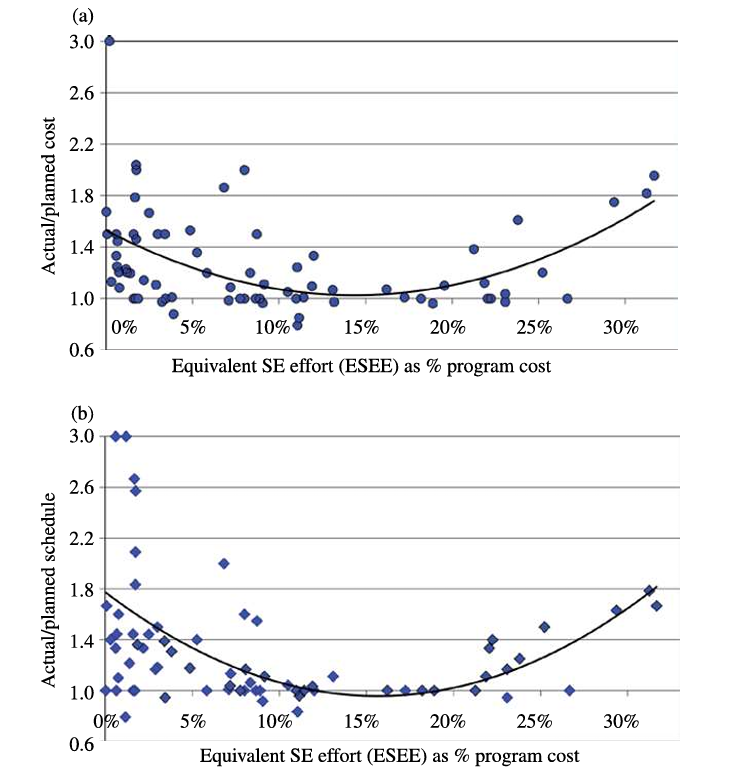
\includegraphics[width=0.48\linewidth]{figs/ch1/cost-schedule-overruns-correlate-with-se.png}
        \label{fig:cost_schedule_overruns_correlation_with_se}
    }
    \hfill
    \subfloat[%
        Project Performance versus SE Capability
        \cite{elm_business_2012, walden_systems_engineering_handbook_2015}%
    ]{%
        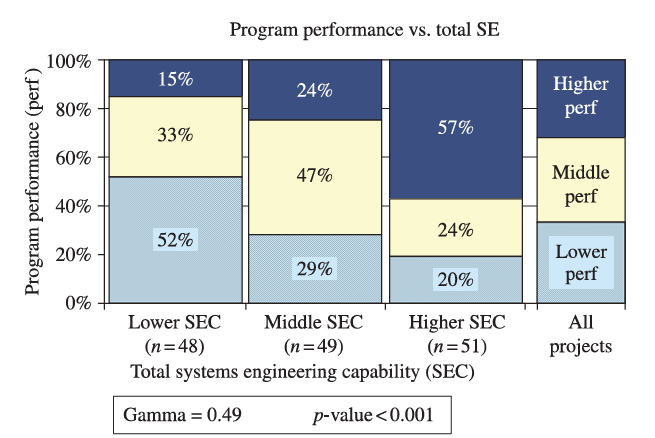
\includegraphics[width=0.48\linewidth]{figs/ch1/program-performance-vs-se.png}
        \label{fig:other_figure}
    }

    \caption{Side-by-side comparison of related figures}
    \label{fig:side_by_side}
\end{figure}


\subsection{The Challenge of Trustworthy AI Usage}

\subsubsection{Failure Modes of LLMs and their Consequences}

Despite the promising benefits of applying \ac{ai} to systems engineering, \acp{llm} introduce critical risks that must be understood and mitigated before deployment in high-stakes environments.

\textbf{Hallucinations.} \acp{llm} can generate plausible-sounding but factually incorrect information with high confidence \cite{Sanu_LLM_Limitations_2024, Furui_Cheng_2024}. In systems engineering contexts, a hallucinated requirement, design constraint, or interface specification could propagate through the lifecycle, compounding errors and increasing rework costs by orders of magnitude. Unlike low-stakes applications where occasional errors are tolerable, \ac{se} decisions directly influence system safety, performance, and cost.

\textbf{Prompt Injection.} Adversarial inputs can manipulate \ac{llm} behavior, causing models to ignore instructions, reveal sensitive information, or produce harmful outputs \cite{Sourav_Banerjee_2024_Vulnerability_LLM_Benchmarks}. For \ac{se} tools that process requirements documents, stakeholder inputs, or legacy system data, prompt injection vulnerabilities pose security risks---particularly when models are integrated into automated workflows.

\textbf{Training Data Contamination.} When benchmark datasets leak into training corpora, models may achieve artificially high scores through memorization rather than genuine reasoning \cite{sainz_nlp_2023, yang_rethinking_2023}. This undermines the validity of benchmark-based evaluations and can lead to overconfidence in model capabilities for domain-specific tasks.

\textbf{Reasoning Opacity.} The ``black-box'' nature of \acp{llm} makes it difficult to trace how conclusions are reached \cite{Johnson2025_Primer_LLM_Limitations}. This conflicts with the traceability requirements fundamental to systems engineering, where architectural decisions must be justified and auditable throughout the system lifecycle.

These failure modes are particularly consequential in defense and safety-critical applications common to systems engineering practice. Many \ac{dod} systems operate in disconnected or air-gapped environments---shipboard systems, tactical networks, and classified enclaves---where cloud-based \ac{llm} services are unavailable and local models cannot receive updates or corrections. In such contexts, the inability to ground model outputs in current, authoritative sources amplifies the risk of hallucinations and outdated reasoning.

The combination of these failure modes prevents the transition from human-in-the-loop to human-on-the-loop operation. Truly agentic \ac{se} assistants---capable of autonomously drafting requirements, generating architecture alternatives, or validating designs---require a level of trust that current evaluation methods cannot yet provide.

\subsubsection{Benchmarking as a Prerequisite for Effective Usage}

Benchmarking is the primary mechanism used across AI research to quantify model capability, compare systems, and build confidence in deployment. The evolution from early benchmarks (WordNet, MNIST, BLEU) to modern high-reasoning datasets (MMLU, ARC, HellaSWAG, BIG-Bench) illustrates how domains progress from simple pattern-matching to complex domain-specific evaluation

Benchmarking is a way to systematically stress-test LLM behavior under known tasks, vocabulary, and reasoning structures before integrating them into operational workflows.

Benchmarking is essential for gauging how well \acp{llm} perform. Given the complexity and high stakes involved in designing and operating large-scale systems, it is crucial to quantitatively and qualitatively assess whether LLM outputs meet the desired standards of accuracy, reliability, and conceptual depth. By comparing \ac{llm} performance to established metrics, human experts, or other AI tools, benchmarking provides a structured mechanism to identify strengths and weaknesses in model capabilities \cite{Tianle_Li_2024_BenchBuilder_ArenaHard_LLM_Benchmarking, Jin_Li_2024_Benchmarking_LLMs_EBM, Muharrem_Unal_2023_HELM_Holistic_Eval_LLMs, Yue_Liu_2023_Reliability_LLMs_Program_Generation}.

Beyond simple metrics, benchmarking also helps guide future \ac{ai} improvements. When engineers and researchers understand where an LLM falls short they can make informed decisions about model selection, tuning, or augmentation. Ultimately, systematic benchmarking ensures that the use of LLMs in systems engineering is grounded in evidence-based practices and aligned with industry and stakeholder needs.

Creating domain-specific benchmarks for any domain is a challenging endeavor as it requires representative datasets, carefully crafted tasks, and contextually relevant metrics. Given that systems engineering contexts are inherently diverse: what matters for a satellite design project may differ dramatically from what is critical for a nuclear submarine’s maintenance schedule. Capturing this diversity in a single benchmark demands careful thought and collaboration among experts who understand the nuances of various engineering subfields. In some cases, a single benchmark may be acceptable while in others, tailored benchmarks for for different use cases may be required. 

Furthermore, the complexity of systems engineering tasks can make isolating measurable performance indicators difficult. Tasks that rely heavily on conceptual reasoning, trade-off analysis, or multi-layered stakeholder requirements prove to be challenging endeavors to reduce to simplistic performance scores. The lack of publicly available, domain-specific corpora further complicates the benchmarking process. As a result, developing robust benchmarks often involves time-consuming data collection and expert annotation to ensure that test sets remain both challenging and accurately represents systems engineering tasks. Other fields have already begun creating domain-specific benchmarks, such as but not limited to the biomedical field \cite{jin_pubmedqa_2019}, medical and clinical field \cite{pal_medmcqa_2022}, legal field \cite{guha_legalbench_2023, chalkidis-etal-2022-lexglue}, and the financial field \cite{xue_famma_2024, islam_financebench_2023}.

However, no equivalent benchmark existed for systems engineering until recently. Generic language benchmarks do not evaluate SE task types, SE vocabulary, MBSE reasoning, lifecycle analysis, or trade-space thinking.

SysEngBench represents a pioneering effort to create a tailored benchmark for evaluating LLMs in systems engineering contexts \cite{bell_rabellsysengbench_2024, Bell2025SysEngBench}. By focusing specifically on the tasks, terminologies, and reasoning patterns intrinsic to the field, SysEngBench attempts to move beyond generic language benchmarks that fail to capture the complexity of systems engineering specific discourse. It seeks to provide a more dedicated measure of how well an \ac{llm} can handle domain-specific challenges.

The nature of progress in AI technologies ensures that new paradigms, methodologies, and technologies will emerge over time, potentially rendering certain aspects of the benchmark more easily performed. The extensibility requirement of the benchmark comes to light as AI technology progresses and SysEngBench must evolve to push the evaluation envelope. Nonetheless, SysEngBench lays the groundwork for a more rigorous and representative approach to evaluating \ac{llm} performance for systems engineers.

Systems engineering integrates tasks like requirements analysis, design synthesis, and risk management to address complex challenges. \acp{llm} can support these workflows by automating documentation and aiding decision-making, with a gamut of models performing well and others not so well with domain-specific tasks on tailored benchmarks such as SysEngBench that uses the \ac{mcq} evaluation modality \cite{Bell2025SysEngBench}. Techniques like quantization further enhance efficiency but require careful trade-offs to maintain accuracy in high-stakes systems engineering applications \cite{Bell2025LLMQuantization}.


\section{The Problem}\label{sec:problem}

\subsection{The Validation Gap in AI Adoption for Systems Engineering}

Systems engineering stands to benefit significantly from \ac{ai}-enabled reasoning assistance, but responsible adoption requires establishing whether models can actually perform \ac{se}-relevant tasks reliably. The core hypothesis is straightforward: if \ac{ai} can accelerate \ac{se} workflows, then \ac{se} performance should improve measurably in cost, schedule, and technical outcomes. Yet no validated pathway exists to verify this claim for the systems engineering domain.

Currently, practitioners can leverage \ac{ai} tools in human-in-the-loop configurations, where humans verify and correct model outputs before they influence decisions. However, achieving human-on-the-loop operation---where truly agentic assistants operate with greater autonomy---requires a foundation of trust. This trust must be established through rigorous validation and verification, specifically through domain-appropriate benchmarks and evaluation methodologies.

\subsection{Research Gap Statement}

Despite the proliferation of \ac{llm} benchmarks across various domains, a critical gap exists in the evaluation of \acp{llm} for systems engineering applications:

\begin{enumerate}
    \item \textbf{Limited domain-specific benchmarks:} While SysEngBench represents a pioneering effort to create \ac{se}-specific evaluation datasets, it currently relies exclusively on \acp{mcq}, which may not fully capture the reasoning depth required for complex \ac{se} tasks \cite{Bell2025SysEngBench}.

    \item \textbf{Unexplored evaluation modalities:} The comparative effectiveness of \acp{mcq} versus \acp{osq} for assessing \ac{llm} performance in \ac{se} contexts remains unstudied. \acp{osq} may reveal reasoning capabilities and limitations that structured \acp{mcq} cannot detect.

    \item \textbf{Unknown cost-performance trade-offs:} The tokenomics and computational costs of different evaluation modalities---particularly when comparing reasoning versus non-reasoning models---have not been characterized for \ac{se} applications.

    \item \textbf{Lack of practical guidance:} Practicing systems engineers lack evidence-based recommendations for selecting appropriate \ac{llm} evaluation approaches for their specific use cases.
\end{enumerate}

\subsection{Research Hypothesis}

This research is guided by the following hypothesis:

\begin{quote}
\textit{If the evaluation modalities of \acp{mcq} and \acp{osq} are systematically compared for systems engineering domain-specific tasks, then \acp{osq} will reveal deeper reasoning capabilities and limitations that \acp{mcq} alone cannot capture, while \acp{mcq} will provide more cost-effective and reproducible baseline measurements. A hybrid approach combining both modalities will yield the most comprehensive assessment of \ac{llm} performance for systems engineering applications.}
\end{quote}

The overarching research question driving this dissertation is: \textit{How do we assess and compare the performance of language models on systems engineering tasks in a rigorous, reproducible, and domain-specific manner, enabling the community to identify strengths, weaknesses, and applicability across \ac{se} processes?}

\section{Research Questions and Objectives}\label{sec:research_questions_objectives}

The focus of this work is to explore, derive, and evaluate methodologies for benchmarking the performance of \acp{llm} in systems engineering. Specifically, this study investigates the comparative effectiveness of \acp{mcq} and textual response formats in evaluating LLMs' understanding and reasoning capabilities in domain-specific tasks. This research also addresses challenges associated with dataset creation, evaluation metrics, and cost considerations. The overarching research questions are as follows:

\begin{itemize}
    \item How do the evaluation modalities of MCQs and textual responses compare in effectively assessing the performance of LLMs in systems engineering?
    \item What are the strengths and limitations of using MCQs as a benchmarking methodology in a specialized domain such as systems engineering?
    \item How can textual response formats better capture the nuanced reasoning and conceptual understanding required for systems engineering tasks?
\end{itemize}

To address these questions, this work performed herein examines foundational challenges in benchmarking LLMs for systems engineering. The answers to the following specific questions will contribute to arriving to potential answers to the dissertation focus:

\begin{itemize}
    \item What is the current state of benchmarking methodologies for LLMs in systems engineering?
    \item What is the role of textual response formats in capturing deeper conceptual understanding compared to MCQs?
    \item How can a systematic approach be developed to convert MCQs into high-quality textual datasets while preserving semantic fidelity?
    \item What evaluation metrics can effectively compare LLM-generated textual responses against reference solutions?
    \item How can insights gained from the comparative evaluation of MCQs and textual responses inform the design of more effective benchmarks for LLMs in systems engineering?
    \item How can existing systems engineering task or concept taxonomies, such as those from the INCOSE Handbook, be leveraged?
\end{itemize}

The goal of this research is to develop an evaluation framework to inform practicing systems engineers on the viability of MCQs and OSQs for the evaluation of LLMs in systems engineering tasks. The framework will evaluate the strengths and limitations of MCQ and OSQ formats as benchmarking modalities for systems engineering tasks. The research aims to quantify how well LLMs capture the unique demands of systems engineering, including the nuanced understanding, conceptual reasoning, and problem-solving capabilities required for the field. To ensure a meaningful and fair comparison, the study will employ methodologies to transform structured MCQs into high-quality textual datasets while preserving semantic fidelity, enabling "apples-to-apples" evaluations between the two modalities.

Additionally, this research seeks to investigate the cost difference between the evaluation modalities. This involves continuing the cost modeling research done for MCQs and applying that to OSQs \cite{Bell2025LLMQuantization}. It would also assist in informing AI cost modeling efforts \cite{madachy_systems_2024, Madachy2024CostModelingAI, Madachy2025AIMaturityCost, Madachy_Bell_Longshore_2025_Generative_AI_SE_Maturity_Cost_Framework}. The ultimate objective is to contribute to the refinement of benchmarking methodologies for LLMs in systems engineering, providing actionable insights into their practical applications, while also addressing foundational gaps in evaluation and dataset creation. This work is expected to inform the systems engineering community on practical, cost effective usage of LLMs for systems engineering domain-specific tasks.


\section{Research Contributions and Benefits to the Body of Knowledge}\label{sec:research_contributions}

This research contributes to the advancement of the evaluation of Large Language Models (LLMs) within the domain of systems engineering. It addresses key gaps in evaluation approaches, dataset creation, and the understanding of performance trade-offs for \acp{llm} in through the comparative analysis of various benchmarking methodologies for the field. The primary focus is on comparing the evaluation modalities of \acp{mcq} and \acp{osq}. Both accuracy and cost will be used in the comparison of the evaluation modalities.

The following contributions align with the research questions identified in Section 1.2, providing insights into the development of more effective benchmarks and the practical applications of \acp{llm} for systems engineers. These contributions lay the groundwork for better understanding of \ac{llm} performance in systems engineering.


\subsection{Task-Modality Alignment Framework for Systems Engineering Evaluation}\label{subsec:Contribution_one}
This research introduces a structured framework that maps systems engineering task types to the evaluation modalities most appropriate for assessing them. For instance, the structured nature of \acp{mcq} provides ease of construction and objectivity, while \acp{osq} may capture deeper reasoning and conceptual understanding. The hypothesis is that there is need for hybrid benchmarks that integrate both modalities for the field of systems engineering to ensure comprehensive evaluation. The framework provides principled guidance for aligning evaluation strategy with systems engineering task-specific demands. Additionally, this research leverages an extensible benchmark design that adapts to evolving \ac{llm} capabilities.

\subsection{Robustness Analysis of MCQ Evaluation Using Distractor Variation for Systems Engineering}\label{subsec:Contribution_two}
Expanding upon prior MCQ-only benchmarking work, this work introduces a robustness testing methodology that systematically rotates the correct answer among multiple distractors \cite{zheng_large_2024}. By measuring performance consistency across these variants, the analysis reveals whether models are demonstrating conceptual understanding or guessing. Accuracy variance becomes a diagnostic metric for MCQ reliability across task types.

\subsection{Extension of SysEngBench with Multi-Format Evaluation Questions} \label{subsec:Contribution_three}
This work expands the SysEngBench dataset to include both Multiple-Choice Questions (MCQs) and Open-Style Questions (OSQs) for core INCOSE defined concepts. An LLM-in-the-loop pipeline converts MCQs into free-text prompts, creating parallel evaluation paths. This dual-format design enables controlled, apples-to-apples comparisons of how different modalities capture model understanding across the same underlying SE knowledge.

\subsection{Comparative Effectiveness of MCQ and OSQ Evaluation Modalities} \label{subsec:Contribution_four}
This research assesses the strengths and limitations of MCQ and OSQ formats for different SE task types. It also proposes hybrid strategies—such as combining a distractor-variant MCQ with consensus-scored OSQs to better understand evaluation accuracy. Results could identify modality preferences by task type, informing more effective domain specific benchmark design.

\subsection{Comparative Tokenomics Cost Analysis Between Reasoning and Non-Reasoning Models for Systems Engineering Applications} \label{subsec:Contribution_five}
This research investigates the computational and economic trade-offs of deploying reasoning-oriented versus standard (non-reasoning) \acp{llm} in systems engineering contexts. By measuring token usage and inference latency across equivalent SysEngBench tasks, the analysis quantifies how reasoning models differ in generation length, step-by-step deliberation, and downstream resource demands. Comparative results reveal how token efficiency and overall cost scale with model reasoning depth, providing evidence for selecting cost-effective evaluation and deployment strategies in systems engineering applications.

\subsection{Evidence-Based Guidance for Practical LLM Integration in Systems Engineering Workflows} \label{subsec:Contribution_six}
This research offers actionable recommendations for applying language models in real-world SE contexts. By identifying which evaluation formats best capture model competence for different types of SE tasks, the study supports reliable AI integration into systems engineering workflows for practicing systems engineers.


\section{Structure of the Dissertation}\label{sec:structure_dissertation}
The outline of this dissertation manuscript serves as a road-map of work to be shared. The dissertation began with the Front Matter, which presents the abstract along with tables and figure lists.

Chapter 1 establishes the motivation for the research, defines the problem, articulates the guiding research questions and objectives, outlines the contributions to the \ac{se} body of knowledge, and concludes with how the dissertation is organized.

Chapter 2 surveys the existing literature on benchmarking large language models, describing the current evaluation landscape and methods. It highlights unique challenges in applying these methods to systems engineering, outlines cross-domain strategies, and discusses experimental design and measurement techniques.

Chapter 3 details the overall research framework, from dataset construction to evaluation procedures and computational methods. It specifies the analytical metrics and methods used to ensure rigorous and reproducible results.

Chapter 4 reports the experimental findings, presenting model performance on both multiple-choice and open-style questions and comparing outcomes across modalities. Statistical analysis and a simple tokenomics analysis of the results is also shared.

Chapter 5 interprets the results, drawing implications for benchmarking methodologies and practical applications in systems engineering and \ac{llm} deployment. It addresses the research’s limitations and outlines opportunities for future research.

Chapter 6 summarizes the key contributions of this dissertation manuscript and reflects on the broader impact to the Systems Engineering community as a whole. It closes with final thoughts and recommendations for subsequent investigations.
